\chapter{Frobenius Data: Statistics at Scale}\label{ch:05}

Sato did not derive the semicircle; he saw it, in point counts of specific curves modulo many primes. Birch and Swinnerton Dyer, at about the same time, found their conjecture in plots of $\log\prod_{p\le x}N_p/p$, with $N_p = \#E(\mathbb{F}_p)$, against $\log\log x$, computed on the EDSAC 2 computer in Cambridge \cite{bsd1965}. Both were statistical observations before they were theorems or programmes. This chapter treats Frobenius data in the same spirit and asks three questions of it. How fast does the empirical law approach the Sato Tate law? What correction at the scale of $\log x$ encodes the rank? How often does a trace take a prescribed value? The first leads to discrepancy, the second to the explicit formula, the third to the Lang Trotter conjecture. For each we state what is proved, what is conjectured, and what our computations show, keeping the distance between a stable statistic and a theorem in view.

\section{Computing traces of Frobenius}

Let $E: y^2 = x^3 + ax + b$ with $a,b\in\Z$ and discriminant $\Delta = -16(4a^3+27b^2) \ne 0$. For a prime $p \nmid 2\Delta$ we have
\[
a_p = p + 1 - \#E(\mathbb{F}_p) = -\sum_{x\in\mathbb{F}_p}\Bigl(\frac{x^3+ax+b}{p}\Bigr),
\]
since each $x$ contributes $1 + \bigl(\frac{x^3+ax+b}{p}\bigr)$ affine points and there is one point at infinity. This gives an $O(p)$ algorithm, adequate for $p$ up to about $10^5$ and convenient for checking.\index{point counting}

Baby step giant step methods reduce the cost to $O(p^{1/4})$ group operations: by Hasse, $\#E(\mathbb{F}_p)$ lies in an interval of length $4\sqrt p$, and one searches it for a multiple $m$ of the order of a random point; Mestre's trick with the quadratic twist makes the answer unique for $p > 229$. Schoof's algorithm \cite{schoof1985} computes $a_p \bmod \ell$ from the action of Frobenius on $\ell$ torsion and recovers $a_p$ by the Chinese remainder theorem in time polynomial in $\log p$; the Elkies and Atkin improvements (SEA) are the method of choice at cryptographic sizes. PARI/GP \cite{pari2023} chooses among these in \texttt{ellap}.

For all primes up to a bound the cost per prime is tiny: the $664{,}577$ traces of $E_1$ below $10^7$ took about $20$ seconds on one core. For much larger ranges Harvey's average polynomial time method \cite{harvey2014} computes $a_p$ for all $p\le X$ at once, at a cost per prime polynomial in $\log X$.

\section{The data sets of this book}

All computations were carried out for this book with PARI/GP and Python, on these data.

\begin{enumerate}
\item $E_1: y^2 = x^3 + x + 1$, discriminant $-496$, conductor $496 = 2^4\cdot31$ (LMFDB label 496.a1 \cite{lmfdb}), without complex multiplication; all $664{,}577$ good primes below $10^7$.
\item $E_2: y^2 = x^3 - x$, complex multiplication by $\Z[i]$, conductor $32$; all good primes below $10^7$.
\item Ramanujan's $\tau(p)/p^{11/2}$ for the $78{,}498$ primes below $10^6$.
\item Two hundred curves $y^2 = x^3 + ax + b$ with integers $a,b$ drawn uniformly from $[-50,50]$ (four curves occur twice), singular curves and curves with complex multiplication being discarded; all good primes $p$ with $5\le p<10^6$, about $7.8\times10^4$ per curve.
\item The curves $11a1$, $37a1$, $389a1$ and $5077a1$ of the Cremona tables, of rank $0$, $1$, $2$ and $3$ (the smallest conductors of these ranks); all odd primes below $10^7$.
\end{enumerate}

Table~\ref{tab:05moments} shows the even moments of the normalised traces. They agree with the Catalan numbers $C_m$ (for $E_1$ and $\tau$) and with the moments $\frac12\binom{2m}{m}$ of the CM law $\mu_{\mathrm{CM}}$ of Section~\ref{sec:04cm} (for $E_2$) to relative errors at most $0.06\%$, $0.73\%$ and $0.14\%$ respectively, in every case within one standard error of the corresponding average of independent draws. For $\tau$, Deligne's bound is visible directly: the largest value of $|\tau(p)|/p^{11/2}$ below $10^6$ is $1.99920$.

\begin{table}[t]\centering\small
\begin{tabular}{rrrrrr}
\toprule
$2m$ & $E_1$ & $\tau$ & $C_m$ & $E_2$ & $\frac12\binom{2m}{m}$\\
\midrule
2 & 1.0000 & 0.9987 & 1 & 0.9995 & 1\\
4 & 1.9994 & 1.9939 & 2 & 2.9980 & 3\\
6 & 4.9976 & 4.9772 & 5 & 9.9916 & 10\\
8 & 13.9930 & 13.9204 & 14 & 34.9642 & 35\\
10 & 41.9808 & 41.7250 & 42 & 125.8514 & 126\\
12 & 131.9488 & 131.0436 & 132 & 461.3908 & 462\\
\bottomrule
\end{tabular}
\caption{Even moments of normalised traces: $E_1$ and $E_2$ over good primes below $10^7$, $\tau(p)/p^{11/2}$ over primes below $10^6$, against the Sato Tate (Catalan) and CM predictions.}\label{tab:05moments}
\end{table}

Write $W_j$ for the Weyl average of $U_j(x_p/2)$ over the good primes $p\le x$ (Chapter~\ref{ch:04}). Since $x^{2m} = \sum_{k=0}^m b_{m,k}U_{2k}(x/2)$ with $b_{m,k} = \binom{2m}{m-k} - \binom{2m}{m-k-1}\ge0$ and $b_{m,0} = C_m$, the $2m$th moment equals $C_m + \sum_{k=1}^m b_{m,k}W_{2k}$. The coefficients sum to $\binom{2m}{m}\sim4^m/\sqrt{\pi m}$, so high moments amplify small errors; for questions of rate the right object is the distribution function.

\section{Discrepancy}\label{sec:05disc}

Let $F_{\mathrm{ST}}(t) = \ST([-2,t])$ and let $F_n$ be the empirical distribution function of the first $n$ normalised traces $x_{p_1},\dots,x_{p_n}$, where $p_1<p_2<\cdots$ are the good primes. The \emph{Kolmogorov discrepancy}\index{discrepancy} is
\[
D_n = \sup_{t\in[-2,2]}\bigl|F_n(t) - F_{\mathrm{ST}}(t)\bigr| .
\]
By Theorem~\ref{thm:04STthm} and the continuity of $F_{\mathrm{ST}}$, $D_n\to0$ for every curve without complex multiplication. The question is the rate.

The classical link between $D_n$ and Weyl sums is the inequality of Erd\H{o}s and Tur\'an \cite{erdosturan1948}.\index{Erd\H{o}s Tur\'an inequality}

\begin{theorem}[Erd\H{o}s and Tur\'an]
There is an absolute constant $C$ such that for any points $u_1,\dots,u_n$ in $\R/\Z$ and any integer $M\ge1$,
\[
\sup_{I}\Bigl|\frac{\#\{j\le n: u_j\in I\}}{n} - |I|\Bigr| \le C\Bigl(\frac{1}{M} + \sum_{h=1}^M \frac1h\Bigl|\frac1n\sum_{j=1}^n e^{2\pi i h u_j}\Bigr|\Bigr),
\]
the supremum being over intervals $I$.
\end{theorem}

An analogue for the Sato Tate measure, with Weyl averages of Chebyshev polynomials $U_m$ in place of exponential sums, was proved by Niederreiter \cite{niederreiter1991}. Combined with bounds for Weyl averages from the analytic properties of $L(s,\Sym^m E)$, it converts zero free regions into rates for $D_n$. In the opposite direction, sharp rates for $D_n$ constrain the zeros.

\begin{theorem}[Akiyama and Tanigawa \cite{akiyamatanigawa1999}; Mazur \cite{mazur2008}]
Let $E/\Q$ be an elliptic curve without complex multiplication. If $D_n = O(n^{-1/2+\varepsilon})$ for every $\varepsilon > 0$, then the Riemann hypothesis holds for $L(s,\Sym^m E)$ for every $m\ge1$.
\end{theorem}

Akiyama and Tanigawa conjectured the rate in the hypothesis and proved the case $m = 1$, the Riemann hypothesis for $L(s,E)$. The extension to all $m$ is stated by Mazur under analytic hypotheses on $L(s,\Sym^mE)$ that the theorem of Newton and Thorne \cite{newtonthorne2021,newtonthorne2021b} now supplies (Chapter~\ref{ch:04}). The argument is short. The function $U_m(x/2)$ has bounded variation on $[-2,2]$ and Sato Tate mean zero, so integration by parts gives $|\sum_{j\le n}U_m(x_{p_j}/2)|\le V_m\,nD_n$, with $V_m$ its total variation, and the hypothesis gives $\sum_{p\le x}U_m(x_p/2)\ll x^{1/2+\varepsilon}$. In the unitary normalisation, with centre $s = \frac12$, partial summation shows that $\sum_pU_m(x_p/2)p^{-s}$ converges on $\Re s>\frac12+\varepsilon$, while the prime powers and the bad primes contribute a function holomorphic on $\Re s>\frac12$. Hence $\log L(s,\Sym^mE)$ continues holomorphically to $\Re s>\frac12+\varepsilon$, and $L(s,\Sym^mE)$ has no zeros there (Exercise~3); since $\varepsilon$ is arbitrary, the functional equation does the rest. Results in the other direction are much weaker. Using the functoriality of Newton and Thorne, Thorner \cite{thorner2021} proved unconditionally that $D_n\ll\log(N\log p_n)/\sqrt{\log p_n}$, with $N$ the conductor of $E$ and an absolute implied constant. For squarefree $N$ and assuming the Riemann hypothesis for every $L(s,\Sym^mE)$, Rouse and Thorner \cite{rousethorner2017} obtained the explicit form $D_n\ll p_n^{-1/4}\log(Np_n)$ of V. K. Murty's bound \cite{murty1985} of order $n^{-1/4}$ up to logarithms, still far from $n^{-1/2}$.

\begin{figure}[t]\centering
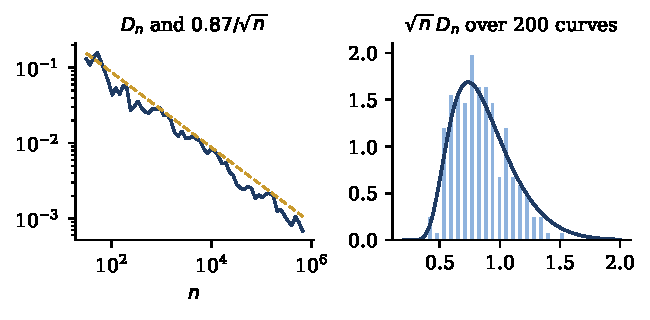
\includegraphics[width=\textwidth]{figs/discrepancy.pdf}
\caption{Left: Kolmogorov discrepancy $D_n$ for $E_1$ against $0.87/\sqrt n$, the asymptotic mean of $D_n$ for $n$ independent draws from $\ST$. Right: histogram of $\sqrt n\,D_n$ over $200$ random curves without complex multiplication (primes below $10^6$) against the density of the Kolmogorov distribution.}\label{fig:05discrepancy}
\end{figure}

\subsection{Our evidence}

For $E_1$ the scaled discrepancy $\sqrt n\,D_n$ equals $0.60$, $0.79$, $0.80$, $0.66$, $0.55$ at $n = 10^2, 10^3, 10^4, 10^5$ and at $n = 664{,}577$ (all good primes below $10^7$). The values stay of order one over almost four orders of magnitude (Figure~\ref{fig:05discrepancy}), as for independent draws; five values of a statistic whose spread under independence is about $0.26$ cannot reveal a slow trend. For $\tau(p)$ over primes below $10^6$ the value is $0.646$.

If the traces were independent draws from $\ST$, Kolmogorov's theorem \cite{kolmogorov1933} would give $\sqrt n\,D_n \Rightarrow K = \sup_{0\le u\le1}|B(u)|$, with $B$ a Brownian bridge (Exercise~2); $K$ has mean $\sqrt{\pi/2}\,\log 2 = 0.8687$, standard deviation $0.2603$, and $10$th, $50$th and $90$th percentiles $0.571$, $0.828$, $1.224$. Over our $200$ random curves, $\sqrt n\,D_n$ has mean $0.837$, standard deviation $0.219$, and percentiles $0.576$, $0.828$, $1.147$. A Kolmogorov Smirnov test of the $200$ values against the law of $K$ gives $p = 0.40$, so it detects no departure from the Kolmogorov law. It has limited power, however, against a contraction of the spread that moves the mean far less than the standard deviation, as here. For $200$ independent copies of $K$ the standard errors of the sample mean and standard deviation are $0.018$ and $0.016$; the observed mean is $1.7$ standard errors below $0.8687$, the standard deviation $2.7$ standard errors below $0.2603$, and the upper tail is visibly lighter (Figure~\ref{fig:05discrepancy}, right). Across curves, the discrepancy at about $7.8\times10^4$ primes has the size expected for independent draws and is, if anything, less dispersed.

\subsection{Interpretation}

Three qualifications apply.

First, the sequence $(x_p)$ is deterministic. A $p$ value of $0.40$ says that a summary of a deterministic object is unremarkable under a reference law; it does not say the object is random. What is random in our experiment is the choice of curve, so the law of $\sqrt n\,D_n$ across curves is a vertical statistic, closer to the family averages of Chapter~\ref{ch:06} than to a statement about one curve.

Second, the explicit formula predicts structure that independent sampling lacks. In the unitary normalisation let $r_m$ be the order of $L(s,\Sym^mE)$ at $s = \frac12$. The prime squares enter through the identity $\tr\Sym^m(g^2) = \sum_{j=0}^m(-1)^j\tr\Sym^{2m-2j}(g)$ (Exercise~4), whose right side has Sato Tate mean $(-1)^m$, and the Riemann hypothesis for $L(s,\Sym^mE)$ gives
\[
\sum_{p\le x}U_m(x_p/2)\log p = -\bigl((-1)^m + 2r_m\bigr)\sqrt x - \sum_{\gamma\ne0}\frac{x^{1/2+i\gamma}}{\frac12+i\gamma} + o(\sqrt x),
\]
with $\gamma$ running over the ordinates of the nontrivial zeros $\frac12+i\gamma$ of $L(s,\Sym^mE)$, counted with multiplicity. By the method of Rubinstein and Sarnak \cite{rubinsteinsarnak1994}, the left side divided by $\sqrt x$ has a limiting distribution in logarithmic scale, with mean $-((-1)^m + 2r_m)$. For $m = 1$, where $r_1 = r$ is the analytic rank of $E$, the mean is $1 - 2r$: this is the rank bias of Section~\ref{sec:05bias}. By partial summation $\sum_{p\le x}U_m(x_p/2)$ is then of order $\sqrt x/\log x$, a factor $\sqrt{\log x}$ below the $\sqrt{\pi(x)}$ of independent sampling. Thus, for each fixed $m$, $\sqrt n\,W_m\to0$ in logarithmic density, $n$ being the number of good primes up to $x$, whereas for independent draws $\sqrt n\,W_m$ is asymptotically standard normal. Since $\sqrt n\,W_m = -\frac12\int_{-2}^2\sqrt n\,(F_n - F_{\mathrm{ST}})(t)\,U_m'(t/2)\,dt$, it follows that under the Riemann hypothesis for every $L(s,\Sym^mE)$ the process $\sqrt n\,(F_n - F_{\mathrm{ST}})$ has no nondegenerate limit in law in logarithmic scale, Brownian bridge or other: every Chebyshev coefficient of a limit would vanish.

The decay is slow, however. The variance of the limiting distribution grows with the logarithm of the analytic conductor of $L(s,\Sym^mE)$, which is at least linear in $m$, and heuristically frequency $m$ is damped only once $\log x$ is large compared with it. Below $10^7$ this can affect only the first few frequencies, consistent with a spread close to that of the Kolmogorov law; whether it accounts for the smaller spread across curves is open. For $E_1$ at $x = 10^7$ the twelve values of $\sqrt n\,W_m$, $m\le12$, have mean square $0.49$ against $1$ for independent draws; a sum of twelve squares of independent standard normal variables falls this low with probability $0.08$, so the data neither confirm nor exclude damping at this scale. The first of them, $-0.36$, may be compared with the leading order prediction $(1-2r)/\sqrt{\log x} = -0.25$ for its mean, $E_1$ having analytic rank $r=1$.

Third, statements at the scale $n^{-1/2}$ are beyond present methods. For independent draws $\sqrt n\,D_n = O(\sqrt{\log\log n})$ almost surely, by the law of the iterated logarithm; for the traces, even $\sqrt n\,D_n = O(n^{\varepsilon})$ for every $\varepsilon>0$ would imply the Riemann hypothesis for every $L(s,\Sym^mE)$, by the theorem above. We state the questions as follows.

\begin{conjecture}[Size of the Sato Tate discrepancy; open]\label{conj:05bridge}
Let $E/\Q$ be without complex multiplication, and let $n$ be the number of good primes up to $x$.
\begin{enumerate}[label=(\alph*)]
\item (Akiyama and Tanigawa.) $D_n = O(n^{-1/2+\varepsilon})$ for every $\varepsilon>0$.
\item $\sqrt n\,D_n\to0$ in logarithmic density: for every $\delta>0$ the set of $x$ with $\sqrt n\,D_n>\delta$ has logarithmic density zero.
\end{enumerate}
\end{conjecture}

Part (b) is our reading of the explicit formula. For each fixed frequency the corresponding statement, $\sqrt n\,W_m\to0$, follows from the Riemann hypothesis for $L(s,\Sym^mE)$, as shown above; the open point is uniformity in $m$, since $D_n$ sees frequencies up to about $\sqrt n$. Part (b) strengthens the conditional statement above that no nondegenerate limit exists along the primes of one curve. Open Problem~\ref{op:disc} of Chapter~\ref{ch:13} asks whether a Brownian bridge arises under another randomisation, for instance over curves of growing conductor, and Computational Problem~\ref{cp:05bridge} proposes a test.

\section{The explicit formula and rank bias}\label{sec:05bias}

Let $E/\Q$ have conductor $N$ and analytic rank $r = \operatorname{ord}_{s=1}L(s,E)$. Write
\[
S(x) = \sum_{p\le x,\ p\nmid N}\frac{a_p\log p}{p} = \sum_{p\le x,\ p\nmid N}\frac{x_p\log p}{\sqrt p}.
\]
For $p\nmid N$ we have $\log(N_p/p) = -a_p/p + (1 - x_p^2/2)/p + O(p^{-3/2})$, and $\sum_{p\nmid N}(x_p^2 - 1)/p$ converges by the prime number theorem for $L(s,\Sym^2E)$; so the asymptotic $\prod_{p\le x}N_p/p\sim A(\log x)^r$ that Birch and Swinnerton Dyer read from their plots \cite{bsd1965} amounts to $\sum_{p\le x,\,p\nmid N}a_p/p = (\frac12 - r)\log\log x + O(1)$. The same prediction with weights $\log p$ is
\[
S(x) \approx \Bigl(\frac12 - r\Bigr)\log x .
\]\index{rank bias}

We explain where the two terms come from. Normalise $L(s,E)$ so that the centre is at $s = 1$ and write $a_p=2\sqrt p\cos\theta_p$. Then
\[
-\frac{L'}{L}(s,E) = \sum_{n}\frac{\Lambda_E(n)}{n^s},\qquad \Lambda_E(p^k) = p^{k/2}\,2\cos(k\theta_p)\log p\quad(p\nmid N).
\]
Assuming the Riemann hypothesis for $L(s,E)$, the explicit formula, applied with a smooth cutoff at the centre, expresses $\sum_{n\le x}\Lambda_E(n)/n$ as $-r\log x$ (the contribution of the zero of order $r$ at $s = 1$) minus a sum over the other zeros $\rho = 1 + i\gamma$, oscillating like $\sum_{\gamma\ne0}x^{i\gamma}/(i\gamma)$, plus a bounded term. The prime terms give $S(x)$. The prime square terms give
\[
\sum_{p\le\sqrt x}\frac{2\cos(2\theta_p)\log p}{p} = \sum_{p\le\sqrt x}\frac{(U_2(x_p/2) - 1)\log p}{p} = -\frac12\log x + o(\log x),
\]
where we used $2\cos2\theta = U_2(\cos\theta) - 1$, Mertens' theorem $\sum_{p\le y}\log p/p = \log y + O(1)$, and the fact that $\sum_{p\le y}U_2(x_p/2)\log p/p = o(\log y)$, which follows from the holomorphy and nonvanishing of $L(s,\Sym^2 E)$ on $\Re s = 1$ in the unitary normalisation (Chapter~\ref{ch:04}). Cubes and higher powers contribute $O(1)$. Hence
\[
S(x) - \frac12\log x = -r\log x - \sum_{\gamma\ne0}\frac{x^{i\gamma}}{i\gamma} + O(1),
\]
heuristically. The $\frac12$ is the shadow of the symmetric square: the prime square coefficient $U_2(x_p/2) - 1$ has average $-1$ over primes because $L(s,\Sym^2E)$ has no pole at $s = 1$. Under the Riemann hypothesis for $L(s,E)$ the oscillatory sum has bounded mean square in $\log x$, so $S(x)/\log x \to \frac12 - r$ in logarithmic mean; a zero off the line would instead produce oscillations of exponential amplitude in $\log x$. The pointwise statement is not known to follow from the Riemann hypothesis, but Kim and Murty \cite{kimmurty2023} showed that if $S(x)/\log x$ has a limit, the limit is $\frac12 - r$. For the product itself, Goldfeld \cite{goldfeld1982} showed that if $\prod_{p\le x}N_p/p\sim A(\log x)^r$ for some $A>0$ and real $r$, where $N_p$ counts the nonsingular points when $p\mid N$, then $L(s,E)$ satisfies the Riemann hypothesis, $r = \operatorname{ord}_{s=1}L(s,E)$, and $A = \sqrt2\,e^{r\gamma_{\mathrm E}}\,r!/L^{(r)}(E,1)$, with $\gamma_{\mathrm E}$ Euler's constant. The factor $\sqrt2$ comes from the same prime squares, which the product cuts off at $p\le x$ rather than at $p^2\le x$; Conrad \cite{conrad2005} relates it to second moments for general $L$ functions. Kuo and Murty \cite{kuomurty2005} and, independently, Conrad showed that the asymptotic for the product is equivalent to $\sum_{n\le x}\Lambda_E(n) = o(x\log x)$, a bound stronger than the $O(x\log^2x)$ that the Riemann hypothesis gives.

\begin{table}[t]\centering\small
\begin{tabular}{lccccc}
\toprule
Curve & $r$ & $\frac12 - r$ & slope & computed $S(10^7)$ & $(\frac12 - r)\log 10^7$\\
\midrule
$11a1$ & 0 & $0.5$ & $0.46$ & $6.46$ & $8.06$\\
$37a1$ & 1 & $-0.5$ & $-0.59$ & $-9.76$ & $-8.06$\\
$389a1$ & 2 & $-1.5$ & $-1.43$ & $-26.73$ & $-24.18$\\
$5077a1$ & 3 & $-2.5$ & $-2.51$ & $-43.54$ & $-40.30$\\
\bottomrule
\end{tabular}
\caption{Rank bias. The slope of $S(x) = \sum_{p\le x}a_p\log p/p$ against $\log x$ is the chord slope $(S(10^7) - S(10^3))/\log 10^4$, compared with $\frac12 - r$. The computed $S$ runs over the odd primes, bad prime included; adding $p = 2$, where $a_2 = -2$ for all four curves, would lower every value of $S$ by $\log 2$ and leave the slopes unchanged.}\label{tab:05bias}
\end{table}

Table~\ref{tab:05bias} and Figure~\ref{fig:05rankbias} show the four curves. The slopes match $\frac12 - r$ to within $0.1$ in every case, and the computed $S(10^7)$ lies below $(\frac12 - r)\log 10^7$ by between $1.6$ and $3.2$, offsets that the explicit formula attributes to the $O(1)$ term and the low lying zeros. The rank is visible with a ruler, and so is the extra $\frac12$.

\begin{figure}[t]\centering
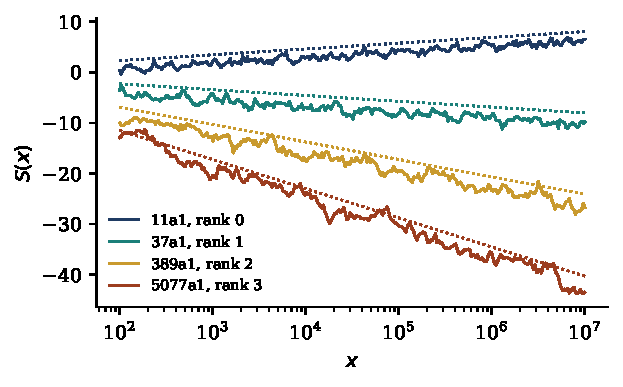
\includegraphics[width=0.85\textwidth]{figs/rankbias.pdf}
\caption{$S(x) = \sum_{p\le x}a_p\log p/p$ for $11a1$, $37a1$, $389a1$, $5077a1$ (ranks $0$ to $3$), $10^2\le x\le 10^7$, summed over odd primes as in Table~\ref{tab:05bias}, against the lines $(\frac12 - r)\log x$.}\label{fig:05rankbias}
\end{figure}

Nothing here bears on the Birch and Swinnerton Dyer conjecture itself: $r$ is the analytic rank, and our data test the explicit formula, not the equality of ranks (known when the analytic rank is at most $1$, by Gross and Zagier \cite{grosszagier1986} and Kolyvagin \cite{kolyvagin1988}).

\section{The Lang Trotter conjecture}

For a fixed integer $t$ let $\pi_{E,t}(x) = \#\{p\le x: p\nmid N,\ a_p = t\}$. When $t = 0$ and $p\ge5$, $a_p = 0$ means that $p$ is a supersingular prime of $E$.\index{Lang Trotter conjecture}\index{supersingular primes}

\begin{conjecture}[Lang and Trotter \cite{langtrotter1976}]
Let $E/\Q$ be without complex multiplication and $t\in\Z$. There is a constant $C_{E,t}\ge0$ such that
\[
\pi_{E,t}(x) \sim C_{E,t}\,\frac{\sqrt x}{\log x},
\]
where for $C_{E,t} = 0$ this means that $\pi_{E,t}(x)$ is bounded.
\end{conjecture}

\subsection{The probabilistic heuristic}

The conjecture concerns a set of primes of density zero, about which Sato Tate says nothing; the heuristic is a local limit version of it. The integer $a_p$ lies in an interval of length $4\sqrt p$, so the lattice spacing is $1$ for $a_p$ and $1/\sqrt p$ for $x_p$. If $x_p$ followed $\ST$ with integrality the only constraint, then
\[
\Prob(a_p = t) \approx \Prob\Bigl(\bigl|x_p - t/\sqrt p\bigr| \le \frac{1}{2\sqrt p}\Bigr) \approx \frac{1}{\sqrt p}\cdot\frac{\sqrt{4 - t^2/p}}{2\pi}\approx \frac{1}{\pi\sqrt p},
\]
since the semicircle density at $0$ is $\frac{1}{2\pi}\cdot2 = \frac1\pi$. Summing over $p$, the expected count is
\[
\sum_{p\le x}\frac{1}{\pi\sqrt p}\approx\frac1\pi\int_2^x\frac{du}{\sqrt u\,\log u} = \frac2\pi\,\pi_{1/2}(x),
\]
where $\pi_{1/2}(x) = \int_2^x du/(2\sqrt u\,\log u)\sim\sqrt x/\log x$, using the prime number theorem in the form that primes near $u$ have density $1/\log u$. This is the shape $c\sqrt x/\log x$ with $c = 2/\pi$.

Congruence conditions correct this. Modulo a prime $\ell$, $a_p$ is the trace of $\Frob_p$ in the mod $\ell$ Galois image $G(\ell)\subset\GL_2(\Z/\ell\Z)$, and by Chebotarev \cite{chebotarev1926} the probability that $a_p\equiv t\pmod\ell$ is $\#\{g\in G(\ell):\tr g = t\}/\#G(\ell)$ rather than $1/\ell$. In the same way the probability that $\ell$ divides $|E(\mathbb F_p)|=p+1-a_p$, the value at $1$ of the characteristic polynomial of $\Frob_p$, is the proportion of elements of $G(\ell)$ with eigenvalue $1$; Koblitz \cite{koblitz1988} built from these proportions his conjecture on the primes $p$ for which $|E(\mathbb F_p)|$ is prime, and Chapter~\ref{ch:flt} reads their complements as the shapes of Gamma laws. By Serre's open image theorem \cite{serre1972} there is an integer $m$ such that the image of Galois in $\GL_2(\hat\Z)$ is the full inverse image of its reduction $G(m)\subset\GL_2(\Z/m\Z)$, and the constant of Lang and Trotter is
\[
C_{E,t} = \frac2\pi\cdot\frac{m\,\#\{g\in G(m):\tr g = t\}}{\#G(m)}\cdot\prod_{\ell\nmid m}\frac{\ell\,\#\{g\in\GL_2(\mathbb{F}_\ell):\tr g = t\}}{\#\GL_2(\mathbb{F}_\ell)}.
\]
The factor at $m$ does not in general split over the primes dividing $m$, because the images modulo different primes can be entangled.

For $t = 0$ and full image $\GL_2(\mathbb{F}_\ell)$ the number of trace zero elements is $\ell^3 - \ell^2$ (Exercise~5), so the factor at $\ell$ is $\ell\cdot\ell^2(\ell-1)/\bigl((\ell^2-1)(\ell^2-\ell)\bigr) = \ell^2/(\ell^2-1)$; for $\ell = 2$ it is $4/3$, as four of the six elements of $\GL_2(\mathbb{F}_2)\cong S_3$ have trace $0$. The mod $2$ image of $E_1$ is all of $\GL_2(\mathbb{F}_2)$, since $x^3+x+1$ is irreducible over $\Q$ with nonsquare discriminant $-31$. If the image of Galois were all of $\GL_2(\hat\Z)$, the constant would be
\[
\frac2\pi\prod_\ell\frac{\ell^2}{\ell^2-1} = \frac2\pi\,\zeta(2) = \frac\pi3\approx1.047.
\]
Over $\Q$ this never happens \cite{serre1972}. For $E_1$ the field $\Q(\sqrt{-31})$ lies in $\Q(E_1[2])$, which contains the square root of the discriminant, and in $\Q(\zeta_{31})\subset\Q(E_1[31])$, so the images modulo $2$ and $31$ are entangled. According to the LMFDB \cite{lmfdb}, $E_1$ is a Serre curve: its image in $\GL_2(\hat\Z)$ has index $2$, the least possible, and is cut out by this single condition. The constant is then a finite computation in $\GL_2(\Z/62\Z)$ (Exercise~5):
\[
C_{E_1,0} = \frac\pi3\Bigl(1 + \frac1{62}\Bigr)\approx1.064.
\]

\subsection{What is known}

The conjecture is open for every curve without complex multiplication and every $t$. Elkies \cite{elkies1987} proved that every elliptic curve over $\Q$ has infinitely many supersingular primes; the lower bounds for $\pi_{E,0}(x)$ that are known are far below $\sqrt x/\log x$. Upper bounds $\pi_{E,t}(x) = O(x^{\theta})$ with $\theta < 1$ follow from effective Chebotarev under the generalized Riemann hypothesis (Serre \cite{serre1981}; Murty, Murty and Saradha \cite{murtymurtysaradha1988}), and averages over families of curves confirm the order $\sqrt x/\log x$ (Fouvry and Murty \cite{fouvrymurty1996} for $t = 0$, David and Pappalardi \cite{davidpappalardi1999} for $t\ne0$). For a curve with complex multiplication half the primes are supersingular, which is why the conjecture excludes such curves.

\subsection{Our counts}

For $E_1$ the supersingular primes begin $3, 17, 179, 227, 523, 1031$. The counts below $x = 10^4, 10^5, 10^6, 10^7$ are $10$, $23$, $79$, $210$, and the ratios $\pi_{E_1,0}(x)/\pi_{1/2}(x)$ are $0.66$, $0.65$, $0.89$, $0.91$ (Figure~\ref{fig:05langtrotter}). At $x = 10^7$, where $\pi_{1/2}(x) = 231.5$, the Poisson standard error of the ratio is $\sqrt{210}/231.5\approx0.06$. The data indicate a constant of order one, above the bare $2/\pi\approx0.64$ and more than two standard errors below $C_{E_1,0}\approx1.064$; the ratio has stayed near $0.9$ since $10^6$. Counts of a few hundred are a consistency check only; Computational Problem~\ref{cp:05lt} asks for counts up to $10^{12}$.

\begin{figure}[t]\centering
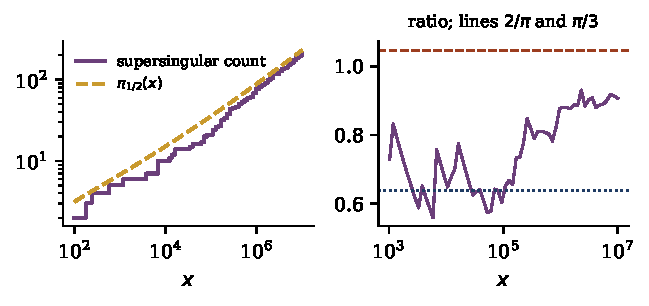
\includegraphics[width=\textwidth]{figs/langtrotter.pdf}
\caption{Supersingular primes of $E_1$ below $10^7$: the count $\pi_{E_1,0}(x)$ against $\pi_{1/2}(x) = \int_2^x du/(2\sqrt u\log u)$ (left), and their ratio (right), with the bare heuristic constant $2/\pi$ and the value $\pi/3$ for a surjective adelic image. The Lang Trotter constant of $E_1$ is $(\pi/3)(1 + 1/62)\approx1.064$.}\label{fig:05langtrotter}
\end{figure}

\section{Notes}

Schoof's algorithm \cite{schoof1985} was the first polynomial time point counting method. Kedlaya and Sutherland \cite{kedlayasutherland2009} computed the distributions of normalised $L$ polynomials of hyperelliptic curves of genus at most $3$ at scale, the numerical side of the classification of Sato Tate groups of abelian surfaces \cite{fkrs2012}. Harvey's average polynomial time method \cite{harvey2014}, made practical by Harvey and Sutherland \cite{harveysutherland2014}, extends such computations much further; Sutherland's survey \cite{sutherland2019} covers the methods, and the LMFDB \cite{lmfdb} holds much of the resulting data. Akiyama and Tanigawa \cite{akiyamatanigawa1999} supported their conjecture with numerical computations of the discrepancy.

The rank bias was implicit in the computations of Birch and Swinnerton Dyer \cite{bsd1965} and made precise by Goldfeld \cite{goldfeld1982}. Sarnak's letter \cite{sarnak2007} treats the biases in the signs of $\tau(p)$ and $a_p$ through all the symmetric powers, and Mazur \cite{mazur2008} discusses the meaning of such error terms. The mechanism is the one behind Chebyshev's bias, where the prime squares produce the bias \cite{rubinsteinsarnak1994}. Chapter~\ref{ch:12} uses the Sato Tate law, with a small atom at $0$ for the supersingular primes, as a likelihood for Bayesian inference.

\section{Exercises}

\begin{enumerate}
\item Prove that $a_p = -\sum_{x\bmod p}\bigl(\frac{x^3+ax+b}{p}\bigr)$ for $p\nmid\Delta$, and deduce that $a_p$ is even if and only if $x^3+ax+b$ has a root modulo $p$. Using the Chebotarev density theorem, compute the proportion of primes with $a_p$ even for $E_1$.
\item Let $Y_1,\dots,Y_n$ be independent with law $\ST$, and let $F_n$ be their empirical distribution function. Show that $\sqrt n\,(F_n - F_{\mathrm{ST}})$ converges in law to $B\circ F_{\mathrm{ST}}$ with $B$ a Brownian bridge, and that $\sqrt n\,D_n\Rightarrow\sup_u|B(u)|$. Verify that $\E\sup_u|B(u)| = \sqrt{\pi/2}\,\log2$.
\item Suppose that $|\sum_{p\le x}U_m(x_p/2)| \le A_m x^{1/2+\varepsilon}$ for all $x\ge2$. Show that the series $\sum_pU_m(x_p/2)p^{-s}$ converges for $\Re s > \frac12+\varepsilon$, and deduce that $L(s,\Sym^mE)$ has no zeros with $\Re s > \frac12 + \varepsilon$ in the unitary normalisation. (Show that the prime powers and the bad primes contribute to $\log L(s,\Sym^mE)$ a function holomorphic on $\Re s>\frac12$.)
\item (Prime squares and bias.) (a) Show that for $g\in\SU(2)$
\[
\tr\Sym^m(g^2) = \sum_{j=0}^m(-1)^j\tr\Sym^{2m-2j}(g),
\]
so that $\tr\Sym^m(g^2)$ has Sato Tate mean $(-1)^m$. (b) Let $x_p$ be independent with law $\ST$. Show that $\sum_{p\le x}x_p\log p/\sqrt p$ has mean $0$ and variance $\sim\frac12\log^2x$, so that a random model without the explicit formula would not produce a drift of size $\frac12\log x$ distinguishable from noise. Explain why the arithmetic sum has much smaller fluctuations.
\item (a) Show that the number of $g\in\GL_2(\mathbb{F}_\ell)$ with trace $t$ is $\ell^3 - \ell^2$ for $t = 0$, and compute it for $t \ne 0$. Deduce the local Lang Trotter factor at $\ell$ for $t\ne0$ when the image is full. (b) Since $E_1$ is a Serre curve, its image in $\GL_2(\hat\Z)$ is the subgroup of index $2$ on which $\operatorname{sgn}(g\bmod2) = \bigl(\frac{\det g}{31}\bigr)$, with $\operatorname{sgn}$ the sign character of $\GL_2(\mathbb{F}_2)\cong S_3$. Show that $C_{E_1,0} = (\pi/3)(1 + e_2e_{31})$, where $e_2$ is the average of $\operatorname{sgn}$ over the trace zero elements of $\GL_2(\mathbb{F}_2)$ and $e_{31}$ that of $\bigl(\frac{\det g}{31}\bigr)$ over the trace zero elements of $\GL_2(\mathbb{F}_{31})$. Show that $e_2 = -\frac12$ and, by counting the solutions of $a^2+bc = -d$, that $e_{31} = -\frac1{31}$, so that $C_{E_1,0} = (\pi/3)(1 + \frac1{62})$.
\item Under the heuristic that the events $\{a_p = 0\}$ are independent with probabilities $C/(2\sqrt p)$, show that $\pi_{E,0}(x)$ has mean and variance both asymptotic to $C\,\pi_{1/2}(x)$ and is asymptotically normal. Using $\pi_{1/2}(10^7) = 231.5$, construct an approximate $95\%$ confidence interval for $C$ from the count $210$ of supersingular primes of $E_1$ below $10^7$, and compare it with $2/\pi$ and with $C_{E_1,0}$.
\end{enumerate}

\section{Open computational problems}

\begin{compproblem}[Brownian bridge test at scale]\label{cp:05bridge}
Objective: test Conjecture~\ref{conj:05bridge}(b) and the predictions for single frequencies in Section~\ref{sec:05disc}, for $E_1$ with all primes up to $10^{10}$ (about $4.6\times10^8$ primes) and for $10^3$ random curves with all primes up to $10^9$. Route: GPU or multicore baby step giant step, or Harvey's average polynomial time algorithm \cite{harvey2014}; streaming accumulation of $F_n$ on a fixed grid and of the Weyl averages $W_m$ for $m\le 100$. Deliverable: plots of $\sqrt n\,D_n$ and of $\sqrt n\,W_m$ against $\log x$, the latter with the means $-((-1)^m + 2r_m)/\sqrt{\log x}$ that the explicit formula predicts; the empirical covariance function of the process at $n = 10^8, 10^9$, compared with $\min(s,t) - st$ after the transform $F_{\mathrm{ST}}$; Kolmogorov Smirnov, Anderson Darling and variance tests of the family values of $\sqrt n\,D_n$ against the law of $K$, with the atom at $0$ created by the supersingular primes treated separately. Why it matters: a decline of $\sqrt n\,D_n$, or of the low frequency Weyl averages, would show the zeros of symmetric power $L$ functions acting on the empirical process and would separate the traces from independent draws; the family test decides whether the smaller spread seen at $10^6$ persists.
\end{compproblem}

\begin{compproblem}[Lang Trotter constants]\label{cp:05lt}
Objective: test the Lang Trotter constants $C_{E,t}$, $t = 0,1,2$, of $E_1$ and of two further Serre curves against counts up to $10^{12}$. Route: adelic images from the LMFDB \cite{lmfdb} and the algorithms of Zywina \cite{zywina2022} and of Rouse, Sutherland and Zureick Brown \cite{rszb2022}; exact evaluation of the Lang Trotter formula by counting in $G(m)$, as in Exercise~5 for $C_{E_1,0}$; counts of $a_p = t$ by testing $(p+1-t)P = O$ for a few random points $P$, much cheaper than computing $a_p$, with hits confirmed by \texttt{ellap}. Deliverable: the constants to six digits; the ratios $\pi_{E,t}(x)/(C_{E,t}\,\pi_{1/2}(x))$ for $x = 10^8,\dots,10^{12}$ with Poisson error bars; a fit of the rate at which they approach $1$. Why it matters: it is the first serious test of the conjecture's constants for these curves, it decides whether the deficit of $E_1$ at $10^7$ is a slow transient, and it measures whether the independence heuristic survives the move from density one statements to density zero ones.
\end{compproblem}

\begin{compproblem}[Bias at high rank]
Objective: check the slope $\frac12 - r$ for curves of rank $4$ to $8$ and beyond, including Elkies's curves of large rank, using all primes below $10^{9}$. Route: curves of rank $4$ to $8$ of small conductor and Elkies's curves, from the LMFDB \cite{lmfdb} and the literature, with $r$ the analytic rank, which for $r\ge4$ is determined only numerically; PARI/GP \texttt{ellap} for the traces; regression of $S(x)$ on $\log x$ with a model for the oscillatory term from the low lying zeros computed by \texttt{lfunzeros} where the conductor permits. Deliverable: a table of fitted slopes against $\frac12 - r$ with confidence bands, and residual plots showing the contribution of the first zeros. Why it matters: for large conductor the oscillatory term is larger and the logarithmic convergence slower, and the data show at what scale the rank becomes legible from Frobenius data alone, a question of practical importance for rank estimation.
\end{compproblem}

\begin{compproblem}[A GPU point counting pipeline]
Objective: build an open pipeline that computes $a_p$ for all primes $p\le10^{10}$ and all curves of conductor up to $10^5$ in the Cremona database, with verification. Route: batched baby step giant step on GPUs with Montgomery arithmetic, cross checked against PARI/GP on random samples and against the Hasse bound and known $L$ values via the approximate functional equation. Deliverable: compressed trace tables, a reproducible build, and timing benchmarks per prime. Why it matters: every statistical question in this chapter and in Chapters~\ref{ch:06} and \ref{ch:12} is limited by data scale, and a shared resource at $10^{10}$ would move discrepancy, bias and Lang Trotter questions into the regime where finite sample effects are small.
\end{compproblem}
